
% Author: Peter Steinbach
\documentclass[tikz]{standalone}
%\documentclass[dvisvgm]{standalone}
%\def\pgfsysdriver{pgfsys-tex4ht.def}
\usepackage{tikz}
\usepackage{units}
\usetikzlibrary{calc,trees,positioning,arrows.meta,chains,shapes.geometric,shapes.arrows,%
    decorations.pathreplacing,decorations.pathmorphing,shapes,%
    matrix,shapes.symbols,fit,backgrounds}

 \pgfdeclarelayer{back}
 \pgfsetlayers{background,back,main}


\makeatletter
\makeatother

\begin{document}


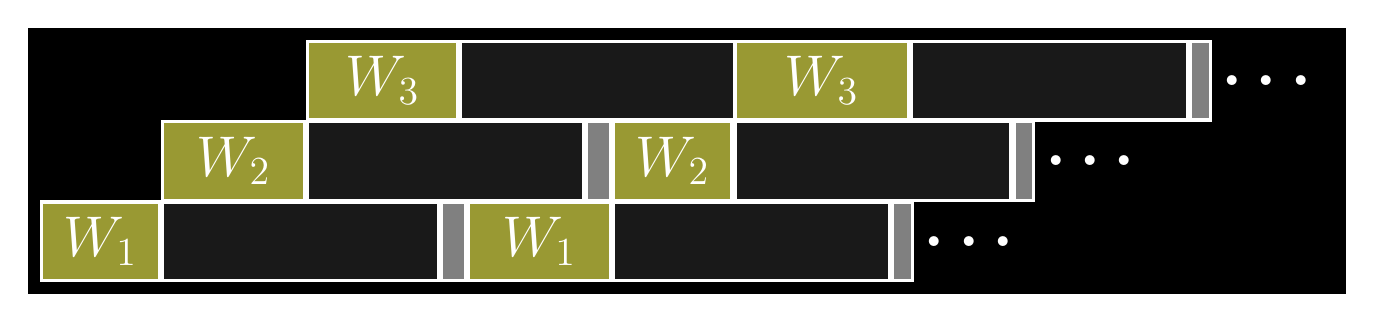
\begin{tikzpicture}[
  show background rectangle, 
  background rectangle/.style={fill=black},
  color=white,
  help lines/.style={color=lightgray,line width=.2pt},
  warp_work/.style={rectangle,very thick,inner sep=0pt,minimum height=1cm,fill=brown!80!green,draw=white,font=\huge,anchor=west},
  warp_delay/.style={rectangle,very thick,inner sep=0pt,minimum height=1cm,fill=gray!20!black,draw=white,font=\huge,anchor=west},
  warp_wait/.style={rectangle,very thick,inner sep=0pt,minimum height=1cm,fill=gray,draw=white,font=\huge,anchor=west}
  ]

%warp 1 
  \node (W_1_a) [warp_work,minimum width=1.5cm] at(0,.5) {$W_{1}$};
  \node (W_1_delay_a) [warp_delay,minimum width=3.5cm] at(W_1_a.east) {};
  \node (W_1_wait_a) [warp_wait,minimum width=.3cm] at(W_1_delay_a.east) {};

  \node (W_1_b) [warp_work,minimum width=1.8cm] at(W_1_wait_a.east) {$W_{1}$};
  \node (W_1_delay_b) [warp_delay,minimum width=3.5cm] at(W_1_b.east) {};
  \node (W_1_wait_b) [warp_wait,minimum width=.25cm] at(W_1_delay_b.east) {};

%warp 2 
  \node (W_2_a) [warp_work,minimum width=1.8cm] at($(W_1_a.north east)+(0,.5)$) {$W_{2}$};
  \node (W_2_delay_a) [warp_delay,minimum width=3.5cm] at(W_2_a.east) {};
  \node (W_2_wait_a) [warp_wait,minimum width=.3cm] at(W_2_delay_a.east) {};

  \node (W_2_b) [warp_work,minimum width=1.5cm] at(W_2_wait_a.east) {$W_{2}$};
  \node (W_2_delay_b) [warp_delay,minimum width=3.5cm] at(W_2_b.east) {};
  \node (W_2_wait_b) [warp_wait,minimum width=.25cm] at(W_2_delay_b.east) {};

%warp 3
  \node (W_3_a) [warp_work,minimum width=1.9cm] at($(W_2_a.north east)+(0,.5)$) {$W_{3}$};
  \node (W_3_delay_a) [warp_delay,minimum width=3.5cm] at(W_3_a.east) {};
%  \node (W_3_wait_a) [warp_wait,minimum width=.5cm] at(W_3_delay_a.east) {};

  \node (W_3_b) [warp_work,minimum width=2.2cm] at($(W_2_b.north east)+(0,.5)$) {$W_{3}$};
  \node (W_3_delay_b) [warp_delay,minimum width=3.5cm] at(W_3_b.east) {};
  \node (W_3_wait_b) [warp_wait,minimum width=.25cm] at(W_3_delay_b.east) {};

  \node (W_3_dots) [font=\Huge,anchor=west] at(W_3_wait_b.east) {\bfseries{}\dots};
  \node (W_2_dots) [font=\Huge,anchor=west] at(W_2_wait_b.east) {\bfseries{}\dots};
  \node (W_1_dots) [font=\Huge,anchor=west] at(W_1_wait_b.east) {\bfseries{}\dots};

  % \node (W_1_b) [rectangle,very thick,inner sep=0pt,minimum width=1.cm,minimum height=1cm,fill=gray,draw=white,font=\huge] at(5.5,.5) {$W_{1}$};
  % \node (W_1_delay_b) [rectangle,minimum width=3.5cm,minimum height=1cm,fill=white!20!black,draw=white,font=\huge] at(2.75,.5) {};


    % \foreach \g in {0,...,2}
%   {
    
%   % \draw[very thick, dashed] ($(-.4,-.4)+(2*\g,0)$) rectangle ($(1.6,2.2)+(2*\g,0) $);

%   \foreach \b in {0,...,2}
%   {
%     \node (number_\b_\g) [rectangle,draw=white,very thick,inner sep=3pt] at ($(0,2)+(.6*\b,0)+(2.2*\g,0)$) {$32$};

%   % \draw[very thick] ($(-.2,1.6)+(.4*\b,0)+(2*\g,0)$) rectangle ($(.2,2.)+(.4*\b,0)+(2*\g,0)$);
%   % \draw [->,very thick,decorate, decoration={snake,amplitude=.4mm,segment length=2mm,post length=1mm}]  ($(0,1.5)+(.4*\b,0)+(2*\g,0)$) -- ($(0,0)+(.4*\b,0)+(2*\g,0)$);

%     \draw [->,very thick,decorate, decoration={snake,amplitude=.4mm,segment length=2mm,post length=1mm}]  (number_\b_\g.south) -- +(0,-2);
% }

% \coordinate (rect_top_right_\g) at($(number_2_\g.north east) + (.2,.2)$);
%   \coordinate (rect_bottom_left_\g) at($(number_0_\g.south west) + (-.2,-2.2)$);
%   \draw[very thick, dashed] (rect_bottom_left_\g) rectangle (rect_top_right_\g);
% }

\end{tikzpicture}
\end{document}
